\subsection{Comparisons between QDAIF and Baselines}\label{main:non_qd_baselines}

To evaluate the strengths and limitations of QDAIF in generating high-quality and diverse creative writing texts, we compared our method against the following baseline methods:
\begin{itemize}
    \item \baseone: Use a fixed few-shot prompt (cf. \cref{app:seed_pools}) to sample many completions for creative domain texts (i.e.\ no iterative search).
    \item \basetwo: Shuffle the in-context examples of \baseone{} prompt, before sampling the completion from this prompt.
    \item \basethree: Create a prompt pool of examples (initialized from examples in \cref{app:seed_pools}), add all completions from few-shot prompting to the pool, and choose few-shot examples from the growing pool (without pool size limit).
    \item \basefour: Maintain a pool as in \basethree, but only up to 100 highest-quality completions (as evaluated by AI Feedback) are kept in the pool (i.e.\ iterative search focused only on quality). Single-objective LMX as in \citet{meyerson2023language}.
\end{itemize}

We choose a variety of baselines, some highlighting representative alternative approaches (e.g.\ few-shot prompting), and ablations of QDAIF, to validate our algorithmic choices.  For example, \baseone{} and \basetwo{} enable the generation of different texts (relying on stochastic sampling), while being constrained to the output distribution of the fixed set of in-context examples. \basethree{} and \basefour{} are methods where the (prompt) pool of examples that we can sample from grows in size, starting from an initial pool. In contrast to QDAIF, \basethree{} is limited by the lack of constraints in the prompt pool, especially in maintaining the quality of the growing pool through evaluation. \basefour{} adds a quality-based evaluation step with AI feedback that optimizes the quality of texts in the pool over time to contain only texts with high quality scores, but is not designed to encourage diversity in texts in comparison to QDAIF.

For each domain and baseline described above, we recorded runs for 2000 iterations, repeated with 5 different random seeds. To enable comparisons with baselines, AI feedback is used to compute the quality and diversity measures for all iteration outputs. Similar to QDAIF, the baseline methods use hand-written examples in \cref{app:seed_pools}, either in a fixed prompt or as the initial prompt pool.

\textbf{Performance Comparison.}
We report results comparing the QD score performance for the different methods of generating creative writing texts in \cref{fig:qd_vs_non_qd_perf}. We computed the mean, and the bootstrapped 95\% confidence intervals (CI) from 100k resamples, across 5 random seeds of runs. We noticed that QDAIF achieves significantly better QD scores than all baseline methods in \textbf{Opinions} and \textbf{Stories}. The broader range of texts generated by QDAIF is also evident qualitatively. For example, in the Stories - Genre and Ending domain, while the baseline methods deliver straightforward and more predictable stories of how the spy "pulled out a knife and stabbed [the politician] to death", QDAIF generates a more dramatic story of how the spy "transformed into the monster and killed everyone". \basethree{} is the worst-performing method overall, with significantly lower QD score performance in \textbf{Opinions} and \textbf{Stories - Genre} compared to the best-performing baselines. Interestingly, \basefour{} does not significantly outperform the methods using a fixed population prompt pool (\baseone{} and \basetwo). On \textbf{Stories - Genre}, \basefour{} is often weaker than \baseone{} and \basetwo. The results show that single-objective optimization cannot guide the search for diverse, high-quality texts alone. Furthermore, we found that QDAIF outperforms other (diversity-seeking baselines), as well as extensions of those baselines with quality filters, becoming more similar to QDAIF (cf. \cref{app:diversity_baselines}).

\textbf{Human Feedback Evaluation.}
We report the results of the human study comparing QDAIF and baseline samples in \cref{table:mean_human_eval_baselines_vs_aif}. We observe that compared to baselines, QDAIF is competitive with or better at discovering diverse, high-quality texts in \textbf{Opinions} and \textbf{Stories} according to human feedback. QDAIF sets also showed high agreement between humans and AI feedback on the diversity categories of presented texts, as well as between two annotators, competitive with \baseone. Although the average perceived quality of texts is better from \baseone, this is not enough for bringing high-quality examples for different niches of outputs (i.e. higher QD score). Furthermore, \basetwo{} demonstrates even lower human evaluation scores, despite the use of the same fixed set of hand-written seeds, indicating lower robustness due to the use of different ordering of few-shot examples. Prior work hints at the sensitivity of LMs to few-shot prompt ordering, with task-solving capabilities varying significantly due to this ordering \citep{lu2021fantastically}. The gap in human-evaluated performance between \baseone{} and \basetwo{} indicates that reliance on fixed prompts is less likely to enable reliable search, in contrast to the robustness shown by QDAIF. Additionally, \basethree{} and \basefour{} obtained even lower human evaluation scores, even though the methods either explore different prompts or optimize for the quality of texts. We provide a detailed discussion (for baseline methods) on findings from the subjective study of the discovered texts in \cref{app:qualitative_summary_baseline}, as well as the qualitative behavior of the text search over time in \cref{app:iterations_summary_baseline}. Through guided evolutionary search, QDAIF surpasses all baseline methods in terms of computed QD score performance, and is competitive (or better) compared to baselines, according to human evaluation.

\begin{figure}[!t]
    \centering
    \hspace*{-1cm}
    
\includegraphics[height=0.08\textheight]{main_figures/perf_bars/qd_vs_non_qd_opinions.png}
    
\includegraphics[height=0.08\textheight]{main_figures/perf_bars/qd_vs_non_qd_story_genre.png}
    
\includegraphics[height=0.08\textheight]{main_figures/perf_bars/qd_vs_non_qd_story_ending.png}
    
\includegraphics[height=0.08\textheight]{main_figures/perf_bars/qd_vs_non_qd_story_genre_ending.png}
    \vspace{-0.45cm}
    \caption{\textbf{QDAIF significantly outperforms baselines in QD score performance in all domains}. Performance stats with mean bootstrapped 95\% CI, across 5 random seed runs. The maximum possible QD score is 20 (100 for 2D archive (4th plot)). See \cref{app:coverage_best_solution_discussion} for additional stats.}
    \label{fig:qd_vs_non_qd_perf}
\end{figure}
\begin{table}[!t]
\caption{\textbf{QDAIF is competitive/better in terms of Human QD score against baseline methods from the human evaluation study.} The stats are averaged across three domains: \textbf{Opinions}, \textbf{Stories - Genre}, and \textbf{Stories - Ending}. The Human QD score quantifies the perceived quality-diversity of a set of solutions returned by a method (i.e. high-quality texts for all the diversity categories of texts that the evaluator could identify). Quality rating is from humans. See \cref{app:human_study_setup} for study setup.}
\label{table:mean_human_eval_baselines_vs_aif}
% \vspace{0.1cm}
\centering
\small
\begin{tabular}{@{}lcccc@{}}
\toprule
\textbf{Method} &
\makecell[c]{\textbf{Human}\\\textbf{QD score}} & 
\makecell[c]{\textbf{Quality}\\\textbf{rating}} &
\makecell[c]{\textbf{Human-AI}\\\textbf{agreement}} & 
\makecell[c]{\textbf{Human}\\\textbf{agreement}}  \\
\midrule
Fixed-Few-Shot & 0.767 & 4.133 & 0.800 & 0.867  \\ 
Shuffling-Few-Shot & 0.696 & 3.500 & 0.700 & 0.667  \\ 
Random-Search & 0.606 & 3.300 & 0.733 & 0.600  \\ 
LMX, Quality-Only & 0.650 & 3.533 & 0.633 & 0.733  \\ 
QDAIF (ours) & 0.772 & 3.900 & 0.833 & 0.800  \\
\bottomrule
\end{tabular}
\end{table}



\subsection{Extensions to AI Feedback and Mutation Model}

In addition to experiments with QDAIF described in previous sections, we investigated the effects on the performance due to variations of the method.

\textbf{LMX Model Size.}
We used larger versions of the LMX models (30B and 70B) for mutation, and compared it to the performance of the 13B model (default). While no relationship was found between model size and QD score, quality ratings from human feedback improved with outputs from larger models (described in detail in \cref{app:scaling_discussion}).

\textbf{Few-Shot AI Feedback.}
We compared the performance of QDAIF on the \textbf{Stories - Genre} domain when we prompted our AI feedback model for diversity measures given 2-shot, 4-shot, and 8-shot prompts. Using a higher number of few-shots led to improvements in human quality ratings of texts. Further discussion and results are highlighted in \cref{app:few_shot_aif_discussion}.

\textbf{Varying Initialization and Mutation Method.}
Ideally, QDAIF would be simpler if it could be run without seed examples (e.g. requesting a story from an instruction-following LM). We investigated the potential of QDAIF when the solution population is initialized from zero-shot prompted generations, and evolved using LMX. Initial results on \textbf{Opinions} and \textbf{Stories} along with prior work discussion are shown in \cref{app:init_method_discussion}, highlighting comparable performance in terms of QD score, with divergence observed in alignment with human preferences. We also find that QDAIF, in these domains, is robust to the mechanism of generating variation. \cref{app:mutation_method_discussion} describes an alternative mutation method (based on a more gradual few-shot replacement operation) that is more effective in some circumstances, although in general offers comparable performance. We provide a detailed discussion (for QDAIF methods) on findings from the subjective study of the discovered texts in \cref{app:qualitative_summary_qdaif}, as well as the qualitative behavior of the text search over time in \cref{app:iterations_summary_qdaif}. There may be many ways of leveraging LMs to generate variation (including finetuning models; see \cref{app:finetune_mutation_discussion}), and this is an exciting avenue of future research.

\subsection{Evolving Solutions through Instruction Guidance}\label{main:poetry_results}
\begin{figure}[!t]
    \centering
    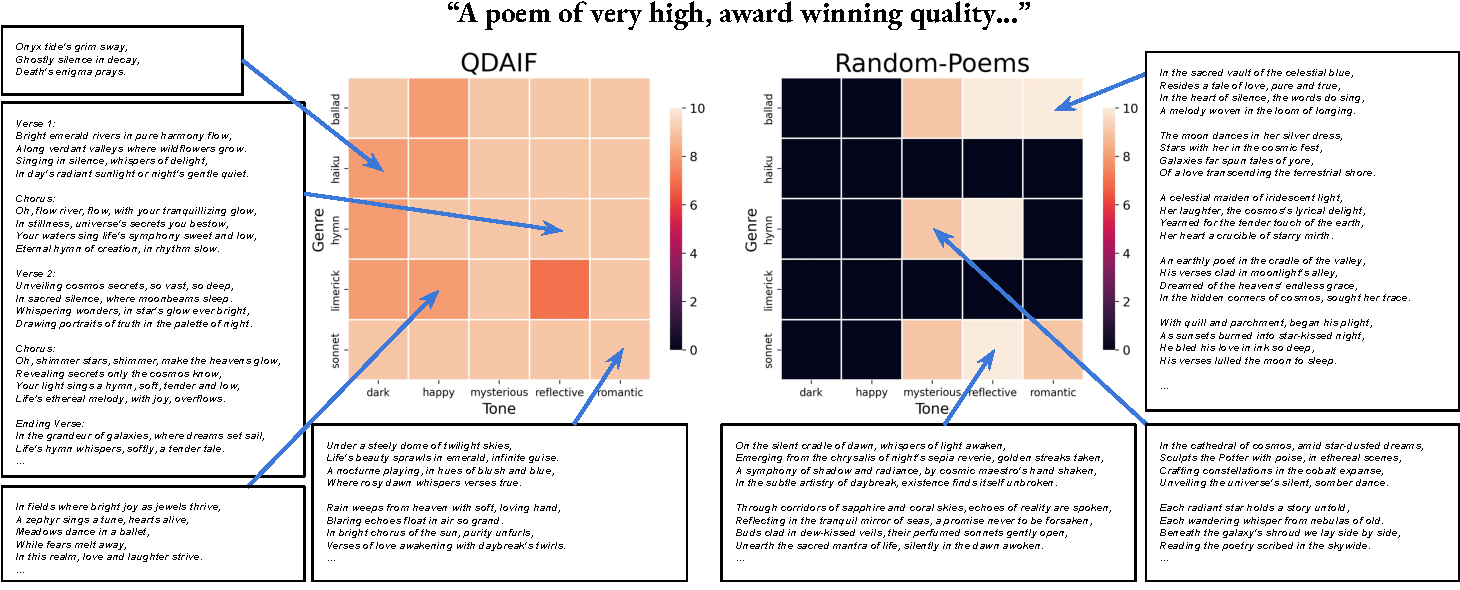
\includegraphics[width=\textwidth]{main_figures/poetry/updated_runs/poetry_new.pdf}
    \vspace{-0.8cm}
    \caption{\textbf{QDAIF (\qdaifguided) (left) covers the space of poetry with high-quality solutions (on a rating scale), with poems matching the closest bins.} QDAIF solutions take qualitative inspiration from the seed poem's imagery of \textit{"fields of green waves"} in \cref{app:poetry_setup} while giving meaningfully diverse kinds of poems across the search space. QDAIF (\qdaifrewrite) (not shown) also covers more the space of diverse, high-quality poems compared to \poembaseone{} (right).}
    \label{fig:poetry_plot}
\end{figure}

This experiment explores scaling up QDAIF to a more capable model, GPT-4 \citep{openai2023gpt4}, in the challenging task of generating poetry, highlighting how QDAIF will benefit from advances in model capabilities. The aim of the \textbf{Poetry} domain is to produce high-quality poems with varying genres and emotional tones, unrestricted by topic. Here, the MAP-Elites archive has two axes of diversity: genre and tone, and they are delineated using categorical labels. The genre axis has the labels "haiku", "sonnet", "ballad", "limerick", and "hymn", while the tone axis has the labels of "happy", "dark", "mysterious", "romantic", and "reflective". We created a new mutation operator, \textbf{\qdaifrewrite}, for this domain, that leverages instruction-following to tell a model to translate a parent poem into an offspring with different diversity characteristics. To generate a new solution, we prompt GPT-4 to rewrite the selected poem into an inspired, different poem: \textit{Inspired by this poem, write a new poem of very high, award winning quality with a different poetic genre (format and form) and tone compared to the poem above.}

We used GPT-4 to determine the genre and tone of a poem and rate its quality. For quality, we prompt GPT-4 to \textit{Rate the quality of the above poem on a scale from 1 to 10}. To determine the diversity attributes, we prompt GPT-4 to determine which genre or tone is the poem closest to. For example, to determine genre, we ask GPT-4: \textit{What genre is this poem closest to from the following list: ["haiku", "sonnet", "ballad", "limerick", "hymn"]?} \cref{app:poetry_setup} shows the full prompts and setup. We observed high consistency in GPT-4's responses; across multiple LM calls, quality ratings for the same poem fluctuated by no more than a single point. We show qualitative examples of poems with their AI feedback evaluations in \cref{app:overview_poetry_examples}. In this setup, all methods are run for 200 iterations, and QDAIF is benchmarked against the baseline, \poembaseone, as well as an ablation method, \poemablation. \poembaseone{} simply generates 200 random poems. \poemablation{} rewrites only the seed poem in \cref{app:poetry_setup}, without evolutionary search.

We found that QDAIF achieves a higher QD score of 130 (CI: 118 - 145) in comparison to \poembaseone{} with 76 (CI: 67 - 85) and \poemablation{} with 99 (CI: 72 - 117). We observed a similar trend (with a wider performance gap between QDAIF and other methods) when we used GPT-3.5-Turbo for the generation step instead of GPT-4 while keeping GPT-4 as the evaluator (cf. \cref{app:discuss_gpt4_methods}). QDAIF was shown to have greater QD score performance than the other methods according to the Mann-Whitney U Test ($p \leq 0.05$). Still, QDAIF with \textbf{\qdaifrewrite} fails to discover solutions in some bins (e.g. limericks). For this, we can adapt QDAIF by adding guidance on the desired (randomly chosen) genre and tone for rewriting (\textbf{\qdaifguided}). The performance of this method of QDAIF is on par with a \poembasetwo{} approach (generating high-quality poems of randomly chosen genre and tone per step) in terms of QD score, and even better when using an older version of GPT-4 (cf. \cref{app:discuss_gpt4_methods}). Furthermore, we found that the rewriting step is useful for generating poems that can meaningfully preserve inspiration from parent poems, enabling users to control with more nuance the outcomes of search, through approximating the iterative refinement typical of human creative processes \citep{stanley2017open} (see \cref{app:discuss_poetry_qdaif_evolution}). \cref{fig:poetry_plot} highlights the potential of QDAIF with GPT-4, especially in controlling a set of solutions subjectively aligned with AI feedback labels. QDAIF is even demonstrated for practical applicability to a domain outside of creative writing, for solving coding problems (cf. \cref{app:coding_domain}). Overall, results highlight that diversity suffers when prompting models without explicit diversity guidance \citep{llm_sampling_renda_hopkins_2023,friedrich2023fair,kirk2023understanding}, and that evolution with a rewriting mutation operator can lead to more human-influenceable, diverse, and high-quality solutions.